\chapter{Results and Analysis}
% (more tables and graphs; comparison; what other people achieved)
The following results and experiments are based upon the AFEW-VA dataset and results will be compared along the metrics Root-Mean-Squared-Error (RMSE) and Pearson Correlation (CORR). The optimization goal is, to reduce the RMSE error, while improving the CORR as much as possible.

\section{Benchmark AFEW-VA Dataset}
In the original paper from 2017, when the AFEW-VA database \citep{Kossaifi:2017:AFEW-VADatabase} was introduced, \citet{Kossaifi:2017:AFEW-VADatabase} already provided a benchmark by comparing different methods, like SVR or DCNN, with the three metrics RMSE (Root Mean Squared Error), CORR (Correlation) and ICC (Interclass Correlation). In the following table, the best performing Deep Neural Network approach is compared with the overall best performing algorithm, called Multiple Kernel Learning (MKL):

\begin{table}[H]
\centering
\begin{tabular}{cc|ccc}
\multicolumn{1}{l}{} & \multicolumn{1}{l|}{\textbf{}} & \multicolumn{1}{l}{\cellcolor[HTML]{CBCEFB}\textbf{RMSE}} & \multicolumn{1}{l}{\cellcolor[HTML]{CBCEFB}\textbf{CORR}} & \multicolumn{1}{l}{\cellcolor[HTML]{CBCEFB}\textbf{ICC}} \\ \hline
FT-DCNN & \cellcolor[HTML]{F8FF00}\textbf{Valence} & 0.37 & 0.26 & - \\
(RGB images) & \cellcolor[HTML]{F8FF00}\textbf{Arousal} & 0.39 & 0.31 & - \\ \hline
MKL & \cellcolor[HTML]{F8FF00}\textbf{Valence} & 0.2639 & 0.401 & 0.274 \\
(Shape+DCT) & \cellcolor[HTML]{F8FF00}\textbf{Arousal} & 0.2229 & 0.445 & 0.34
\end{tabular}
\end{table}

The best performing method compared in this paper is the MKL which performs best in comparison to other methods examined in this paper. In this method the authors utilized different kernels for each, shape features (Norm-shape) and appearance features (Hybrid-DCT).
\newline\newline
The FT-DCNN model, a fine tuned Deep Convolutional Neural Network follows a very similar approach as the one proposed here in this Master thesis. The model is trained on randomly sampled frames from video sequences (just like in this thesis). Fine tuning is being done with AlexNet, a pre trained model on the ImageNet dataset.
\newline\newline
\citet{Theagarajan:2018:DeepDriver} in their 'DeepDriver' paper used the AFEW-VA database to evaluate their approach. It consisted of taking multiple frames as a sequence and feeding them into either a CNN-only architecture, as well as an CNN + LSTM architecture. Both methods heavily outperformed all benchmark results on the RMSE and CORR metric. The best result, using the CNN + LSTM, achieved the following results:


\begin{table}[H]
\centering
\begin{tabular}{c|cc}
\multicolumn{1}{l|}{\textbf{}} & \multicolumn{1}{l}{\cellcolor[HTML]{CBCEFB}\textbf{RMSE}} & \multicolumn{1}{l}{\cellcolor[HTML]{CBCEFB}\textbf{CORR}} \\ \hline
\cellcolor[HTML]{F8FF00}\textbf{Valence} & 0.093 & 0.639 \\ \hline
\cellcolor[HTML]{F8FF00}\textbf{Arousal} & 0.087 & 0.626 \\ 
\end{tabular}
\end{table}

These results were obtained using a 3-fold cross validation approach for training and evaluation. However, the author utilized two different datasets, the AFEW-VA and MotorTrend's dataset. Therefore, there training is being conducted on two separate datsets, which makes this approach not objectively comparable to the approach proposed in this Master thesis. 
\newline\newline
\citet{Handrich:2020:SimultaneousPredVA} made use of cross-database validation for the recognition of valence and arousal in videos/images. They used the AFEW-VA database \citep{Kossaifi:2017:AFEW-VADatabase} as a validation dataset and achieved much better results for the CORR and ICC metrics. This shows that their approach is indeed an improvement to the 2017 benchmark paper. Their proposed CNN architecture is also based upon RGB images as an input and achieves the following results:

\begin{table}[H]
\centering
\begin{tabular}{cl|cc}
\multicolumn{1}{l}{} & \textbf{} & \multicolumn{1}{l}{\cellcolor[HTML]{CBCEFB}\textbf{RMSE}} & \multicolumn{1}{l}{\cellcolor[HTML]{CBCEFB}\textbf{CORR}} \\ \hline
\begin{tabular}[c]{@{}c@{}}AFEW-VA\\ database\end{tabular} & \multicolumn{1}{c|}{\cellcolor[HTML]{F8FF00}\textbf{Valence}} & 0.26 & 0.39 \\
only & \multicolumn{1}{c|}{\cellcolor[HTML]{F8FF00}\textbf{Arousal}} & 0.25 & 0.29 \\ \hline
\begin{tabular}[c]{@{}c@{}}Cross-\\ database\end{tabular} & \cellcolor[HTML]{F8FF00}\textbf{Valence} & 0.28 & 0.58 \\
validation & \cellcolor[HTML]{F8FF00}\textbf{Arousal} & 0.26 & 0.46
\end{tabular}
\end{table}

These results were obtained using 5-fold cross validation on the AFEW-VA database, while training on 70 percent and validating on 30 percent of the whole dataset. Thus, the results are comparable to the herein mentioned approach. Looking closer at their results, an interesting behavior is visible: While the CORR metric increased substantially when using the Cross-database validation, the RMSE metric on the other hand did slightly worse than the training on the AFEW-VA database only.
\newline\newline
The following graph illustrates the results from all the methods tested by \citet{Kossaifi:2017:AFEW-VADatabase} together with the results achieved by \citet{Handrich:2020:SimultaneousPredVA}. The results from \citet{Handrich:2020:SimultaneousPredVA} are marked as 'Pr. CNN', as this graph is taken out of their paper:

\begin{figure}[H]
  \begin{center}
  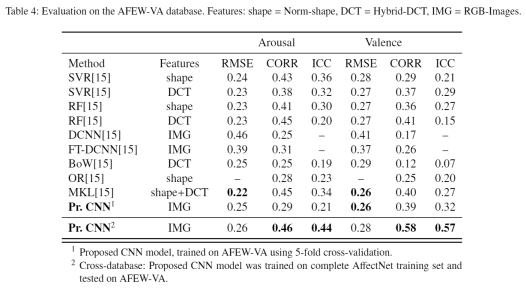
\includegraphics[angle=0, width=0.9\textwidth]{Figures/benchmark.PNG}
  \caption{Benchmark from the paper 'Simultaneous Prediction of Valence/Arousal and Emotions on AffectNet, Aff-Wild and AFEW-VA' \citep{Handrich:2020:SimultaneousPredVA}}
  \label{fig:BenchmarkOnAFEW-VA}
  \end{center}
\end{figure}

It can be clearly seen that the proposed CNN approach by \citet{Handrich:2020:SimultaneousPredVA} easily outperforms the results of Neural Network based approaches (DCNN and FT-DCNN) by \citet{Kossaifi:2017:AFEW-VADatabase}. Only when comparing the results to the best performing algorithm, Multiple Kernel Learning (MKL), in terms of RMSE it reveals a slightly higher loss.


%%%%%%%%%%%%%%%%%%%%%%%%%%%%%%%%%%%%%%%%%%%%%%%%%%%%%%%%%%%

\section{Results}
The results for the approach proposed in this Master thesis were achieved by shuffling data while making sure that training, validation and testing data stays subject-independent. 
\newline\newline
The following two graphs display the learning curves during training for the selected metrics, namely RMSE and CORR, for the predicted Valence values. Subsequently, the respective learning curves are presented for the predicted Arousal values.

\hl{Learning Curve RMSE - Valence}

% \begin{figure}[H]
%   \begin{center}
%   \includegraphics[angle=0, width=0.9\textwidth]{Figures/xx.png}
%   \caption{RMSE metric - Learning curve for Valence}
%   \label{fig:RMSEValence}
%   \end{center}
% \end{figure}

\hl{Learning Curve CORR - Valence}

% \begin{figure}[H]
%   \begin{center}
%   \includegraphics[angle=0, width=0.9\textwidth]{Figures/xx.png}
%   \caption{CORR metric - Learning curve for Valence}
%   \label{fig:CORRValence}
%   \end{center}
% \end{figure}

\hl{Learning Curve RMSE - Arousal}
% \begin{figure}[H]
%   \begin{center}
%   \includegraphics[angle=0, width=0.9\textwidth]{Figures/xx.png}
%   \caption{RMSE metric - Learning curve for Arousal}
%   \label{fig:RMSEArousal}
%   \end{center}
% \end{figure}

\hl{Learning Curve CORR - Arousal}
% \begin{figure}[H]
%   \begin{center}
%   \includegraphics[angle=0, width=0.9\textwidth]{Figures/xx.png}
%   \caption{CORR metric - Learning curve for Arousal}
%   \label{fig:CORRArousal}
%   \end{center}
% \end{figure}


All these graphs show a similar behaviour: While the training curve looks optimal, the validation curve only improves slightly and fails to align with the training curve. Therefore, these results might indicate that the trained model is Overfitting on the training data. However, different architecture and hyper-parameter settings did not lead to any improvements in the evaluation on the testing data.
\newline\newline
The final results were achieved by using the design choices presented in this Master thesis and conduct a 5-fold cross-validation with subject-independent data. The following results represent the average of the results obtained during each of the 5-fold cross-validation:

\begin{table}[H]
\centering
\begin{tabular}{clll}
\multicolumn{1}{l}{\textbf{}} & \cellcolor[HTML]{9aff99}\textbf{ACC} & \cellcolor[HTML]{9aff99}\textbf{RMSE} & \cellcolor[HTML]{9aff99}\textbf{CORR} \\
\cellcolor[HTML]{F8FF00}\textbf{\begin{tabular}[c]{@{}c@{}}Valence\end{tabular}} & 0.28 & 0.27 & 0.22 \\ \hline
\cellcolor[HTML]{F8FF00}\textbf{\begin{tabular}[c]{@{}c@{}}Arousal\end{tabular}} & 0.10 & 0.25 & 0.27
\end{tabular}
\end{table}



%%%%%%%%%%%%%%%%%%%%%%%%%%%%%%%%%%%%%%%%%%%%%%%%%%%%%%%%%%%%%
\section{Comparison}
The following table gives an overview of the results obtained by \citet{Kossaifi:2017:AFEW-VADatabase},  \citet{Handrich:2020:SimultaneousPredVA} and by the approach proposed in this thesis. All the results are directly comprabale as they where achieved by performing the a 5-fold cross-validation with subject independent data between folds.

\begin{table}[H]
\begin{center}
\begin{tabular}{|cc|cc|cc|}
\hline
\rowcolor[HTML]{FCFF2F} 
\multicolumn{1}{|l}{\cellcolor[HTML]{FCFF2F}} & \textbf{Method} &  \textbf{\begin{tabular}[c]{@{}c@{}}RMSE\\ Valence\end{tabular}} & \textbf{\begin{tabular}[c]{@{}c@{}}CORR\\ Valence\end{tabular}} & \textbf{\begin{tabular}[c]{@{}c@{}}RMSE\\ Arousal\end{tabular}} & \textbf{\begin{tabular}[c]{@{}c@{}}CORR\\ Arousal\end{tabular}} \\ 
\hline
\textbf{\begin{tabular}[c]{@{}c@{}}RESULTS\\ THESIS\end{tabular}} & \begin{tabular}[c]{@{}c@{}}FT-DCNN\\ (VGGFace)\end{tabular} & 0.27 & 0.22 & 0.25 & 0.27 \\
\textbf{\begin{tabular}[c]{@{}c@{}} \\ AFEW-VA \\ \citep{Kossaifi:2017:AFEW-VADatabase} \end{tabular}} &
\begin{tabular}[c]{@{}c@{}}FT-DCNN\end{tabular} & 0.37 & 0.26 & 0.39 & 0.31 \\
\textbf{\begin{tabular}[c]{@{}c@{}} \\ Sim. prediction of VA \\ \citep{Handrich:2020:SimultaneousPredVA}\end{tabular}} & CNN & 0.26 & 0.39 & 0.25 & 0.29 \\ \hline
\end{tabular}
\end{center}
\end{table}

The results clearly show that the approach proposed in this Master thesis is substantially outperforming the results obtained by \citet{Kossaifi:2017:AFEW-VADatabase} in terms of Root-Mean-Squared-Error loss. It shows that RMSE is lower by 0.1 for valence and 0.14 for arousal, while the Correlation is lower by 0.04 for valence and 0.04 for arousal. In comparison to the approach proposed by \citet{Handrich:2020:SimultaneousPredVA} the thesis's results were pretty similar for RMSE, but worse for the CORR with 0.17 lower for valence and 0.02 lower for arousal.
\newline\newline
In conclusion, it can be said that the results of this thesis are up to date with the state-of-the-art proposed by \citet{Handrich:2020:SimultaneousPredVA} in \citeyear{Handrich:2020:SimultaneousPredVA} for Emotion Recognition In-The-Wild with the AFEW-VA dataset \citep{Kossaifi:2017:AFEW-VADatabase}. The results also show that fine-tuning a state-of-the-art pre-trained Neural Network is a very decicive factor in beating current state-of-the-art Machine Learning challenges. Furthermore, it is very likely that with further optimization, the proposed approach will even outperform the state-of-the-art.

\subsubsection{FaceReader application}
The FaceReader product of the company Noldus\citep{Noldus:2020:Facereader} is an application that is optimized for researchers to recognize emotions of participants. They make use of the categorical approach, but also convert them into values for valence and arousal. However, their approach is designed for laboratory conditions, thus they demand that the camera is placed slightly below eye-level and that there is no shadow in the person's face. Therefore, there claimed accuracy with 98 percent cannot be compared to In-The-Wild data. As confirmed through an experiment conducted by the author of this thesis, the FaceReader application failed to detect faces in every third (3 out of 9 seconds) due to imperfect conditions with a not perfectly illuminated room.
% However, as mentioned in the Quick Setup Guide, there approach is based upon the premise that the camera is placed slightly below eye-level of the test person and that good lightning, without shadow in the test person's face is crucial. Therefore, there claimed accuracy (from a phone call) with 98 percent cannot be compared to In-The-Wild data with imperfect conditions.
% Through a trial period the product was tested. As a camera an off-the-shelf integrated laptop camera was used in an weakly illuminated room. During the trial period the author realized, that the FaceReader often failed to provide information on expression intensity due to mostly not being able to find a face or also due to bad image quality. In total, in a 9 second experiment it was only able to detect the emotions during 3 of those 9 seconds.


%%%%%%%%%%%%%%%%%%%%%%%%%%%%%%%%%%%%%%%%%%%%%%%%%%%%%%%%%%%%%%%%
\section{Experiments}
Experiments are done with the approach of 'Ablation study'. This means each experiment analyzes a part of the implementation through leaving it out and comparing the results with the former proposed model.\newline
Basis for this is the 5-fold cross-validation approach with subject independent testing and validation data, as it was done by the benchmark papers.

%%%%%%%%%%%%%%%%%%%%%%%%%%%%%%%%%%%%%%%%%%%%%%%%%%%%%%%%%%%%%%%%
\subsection{Experiment 1: MTCNN (Multi-task Cascaded Convolutional Neural Network)}
\textbf{- How often does MTCNN fail to detect faces??}\newline
Out of 30051 frames it only failed to detect a face in 961 faces, this presents 3.2 percent of all images.
\newline\newline
\textbf{- What happens when not using MTCNN and directly feeding the original images into the VGGFace model for fine tuning.}\newline
The model performance slightly increased

\subsection{Experiment 8: Frames where no image is being detected}
So far feeding in the original image, in case MTCNN can't detect a face
-> what happens when deleting the image and not including it in the training data

\subsubsection{Optional: With MTCNN , but instead of keeping the Originalwhen no face was detected -> instead discarding this pair of (image, label)}

%%%%%%%%%%%%%%%%%%%%%%%%%%%%%%%%%%%%%%%%%%%%%%%%%%%%%%%%%%%%%%%%
\subsection{Experiment 2: Data Augmentation}
 In comparison to the results mentioned above, adding data augmentation couldn't show any improvement in performance.
\newline\newline
This data augmentation was applied:
-
\newline\newline
These are the results for the rmse metric for valance and arousal:
No improvement detected

%%%%%%%%%%%%%%%%%%%%%%%%%%%%%%%%%%%%%%%%%%%%%%%%%%%%%%%%%%%%%%%%
\subsection{Experiment 3: Regularization}
\textbf{Which regularization techniques can be applied to provide further improvements on the model performance in terms of loss reduction?}
\textbf{- Dropout layer}
\newline\newline
\textbf{- BatchNormalization layer}\newline
- BatchNormalization layer proved to provide constantly significant better results.
\newline\newline
\textbf{- Model architecture}\newline
- Despite \citet{Pittaras:2017:FineTuningStrategiesComparison} arguing that generally the best approach for finetuning is to only add one Dense Layer with a high number of neurons to the original pretrained model, the obtained results weren't automatically performing better, mostly worse.
\newline\newline
\textbf{- L2 regularization on pretrained model}\newline
Validation loss during training is lower than the training loss, which is very likely because of the reason that regularization was applied. This L2 regularization is only applied during training, but not validation/testing, which explains the significant difference between those values.
https://www.pyimagesearch.com/2019/10/14/why-is-my-validation-loss-lower-than-my-training-loss/

%%%%%%%%%%%%%%%%%%%%%%%%%%%%%%%%%%%%%%%%%%%%%%%%%%%%%%%%%%%%%%%%
\subsection{Experiment 4: LSTM}
\textbf{- Can an LSTM capture the time-spatio changes between frames and thus enhance the performance of \gls{ER}}
Data needs to be non-shuffled in order to do that
-> Performance didn't increase



%%%%%%%%%%%%%%%%%%%%%%%%%%%%%%%%%%%%%%%%%%%%%%%%%%%%%%%%%%%%%%%%
\subsection{Experiment 5: Landmarks from ASM (Active Shape Model)}
\textbf{- Can an AAM decrease the loss of the model performance?}
\newline\newline
\textbf{- How much longer does the program need to run through for one image with an AAM?}
\newline\newline
Construction of landmarks for the whole dataset of 30051 images. From 7402 images it could not detect the face (with dlib face detector)
\newline\newline
As described by \citet{Gao:2010:ActiveAppearanceModels} in an a summarizing paper, called 'Overview of Active Appearance Models', this approach is very suitable for the extraction of compact features in various application. However, they admit that this approach can't satisfy real-time requirements sufficiently, due to its time consuming fitting process.
\newline\newline
This consideration let to the decision to first implement a fast performing algorithm for the task of landmark prediction, instead of an Active Appearance Model which needs for each face a few seconds to be fitted. The decision fell on the algorithm of 'Ensemble of Regression Trees(ERT)' \citep{Kazemi:2014:ShapePredictor} implemented as a pre-trained shape predictor by the dlib library.
\newline\newline
Pre-trained shape predictor from dlib library, proposed by \citet{Kazemi:2014:ShapePredictor} in order to predict 68 facial landmarks. The author also argues that the approach 'Ensemble of Regression Trees (ERT)' is better than Active Shape Model approaches. A comparison between two variants of Active Shape Models the proposed ERT approach show that ERT cuts in half the error of the Active Shape Model variants.
\newline\newline
The 'default' face detector from dlib fails to detect 7402 out of 30051 images, while the MTCNN only fails in 961 images to detect a face. => A logical conclusion would be to use MTCNN to detect the face and the respective bounding box while using the dlib shape predictor, based upon the ERT approach, to time-efficiently detect  facial landmarks.
\newline\newline
\subsubsection{Landmarks only}
When feeding only landmarks into a model with Dense layers there was no improvement.
Even when the units of the Dense layers were drastically increased there was no improvement in terms of training, as well as validation loss. As a result, this experiment showed that with the coordinates of landmarks alone, the Neural Network is not able to predict emotions.

\subsubsection{Combination of images and landmarks}
\textbf{Performance improvement}


%%%%%%%%%%%%%%%%%%%%%%%%%%%%%%%%%%%%%%%%%%%%%%%%%%%%%%%%%%%%%%%%
\subsection{Experiment 6: Heatmap from ASM (Active Shape Model)}

\textbf{Comparison ASM: Landmarks vs. Heatmap}
- considerations run-time per image/batch
- validation/testing loss improvement

%%%%%%%%%%%%%%%%%%%%%%%%%%%%%%%%%%%%%%%%%%%%%%%%%%%%%%%%%%%%%%%%
\subsection{Experiment 7: Heatmap from AAM (Active Appearance Model)}
\textbf{Comparison ASM vs. AAM}
- considerations run-time per image/batch
- validation/testing loss improvement

